\documentclass[11pt]{article}

\usepackage{fullpage}
\usepackage{graphicx}
\usepackage{amsmath}
\usepackage{amssymb}
\usepackage{amsthm}
\usepackage{fancyvrb}

\parindent0in
\pagestyle{plain}
\thispagestyle{plain}

\newcommand{\myname}{Mehshan Mustafa}
\newcommand{\dated}{\today}

\newenvironment{theorem}[2][Theorem]{\begin{trivlist}
\item[\hskip \labelsep {\bfseries #1}\hskip \labelsep {\bfseries #2.}]}{\end{trivlist}}
\newenvironment{lemma}[2][Lemma]{\begin{trivlist}
\item[\hskip \labelsep {\bfseries #1}\hskip \labelsep {\bfseries #2.}]}{\end{trivlist}}
\newenvironment{exercise}[2][Exercise]{\begin{trivlist}
\item[\hskip \labelsep {\bfseries #1}\hskip \labelsep {\bfseries #2.}]}{\end{trivlist}}
\newenvironment{problem}[2][Problem]{\begin{trivlist}
\item[\hskip \labelsep {\bfseries #1}\hskip \labelsep {\bfseries #2.}]}{\end{trivlist}}
\newenvironment{question}[2][Question]{\begin{trivlist}
\item[\hskip \labelsep {\bfseries #1}\hskip \labelsep {\bfseries #2.}]}{\end{trivlist}}
\newenvironment{corollary}[2][Corollary]{\begin{trivlist}
\item[\hskip \labelsep {\bfseries #1}\hskip \labelsep {\bfseries #2.}]}{\end{trivlist}}
\newenvironment{solution}{\begin{proof}[Solution]}{\end{proof}}
\newenvironment{idea}[2][Proof Idea.]{\textit{#1} #2}

\begin{document}

\textbf{Introduction to the Theory of
Computation}\hfill\textbf{\myname}\\[0.01in]
\textbf{Chapter 1: Regular Languages}\hfill\textbf{\dated}\\
\smallskip\hrule\bigskip

\begin{problem}{1.67}
Let the rotational closure of language $A$ be $RC(A) = \{yx \; | \; xy \in A\}$.
\end{problem}

\begin{problem}[Part]{a}
Show that for any language $A$, we have $RC(A) = RC(RC(A))$.
\end{problem}

\begin{proof}
To show that for any language $A$, $RC(A) = RC(RC(A))$, we show that all possible rotations of a string and all possible rotations of a rotation generate the same set of strings.
\\
\\
Let $A$ be any language, and $w$ be any member of $A$. Let $n$ be the length of $w$, then $RC(A)$ contains all of the $n$ possible rotations of the string $w$, which are:
\begin{align*}
&w_{1} w_{2} w_{3} \cdots w_{n-1} w_{n}, \\
&w_{2} w_{3} \cdots w_{n-1} w_{n} w_{1}, \\
&w_{3} \cdots w_{n-1} w_{n} w_{1} w_{2}, \\
&\vdots \\
&w_{n} w_{1} w_{2} w_{3} \cdots w_{n-1}
\end{align*}
Every  $w_{i}$ in above strings is the $i^{th}$ symbol of $w$. All of these strings share the same set of rotations.
\end{proof}

\newpage 

\begin{problem}[Part]{b}
Show that the class of regular languages is closed under rotational closure.
\end{problem}

\begin{idea}
Let $\Sigma = \{0, 1\}$, and define
\[
A = \{w \ | \ w \ contains \ at \ least \ one \ 1 \ and \ an \ even \ number \ of \ 0s \ follow \ the \ last \ 1\}.
\]

\begin{center}
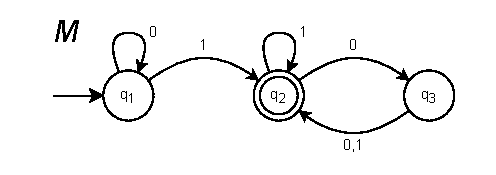
\includegraphics[scale=1.0]{Figures/Problem1.67a.pdf} \\
State diagram of DFA $M$ that recognizes $A$.
\end{center}

Take for example the string $100$, which is a member of $A$, and $M$ accepts $100$ by transitioning through the sequence of states $q_{1},q_{2},q_{3},q_{2}$. The string $010 \in RC(A)$, because it is a rotation of $100$ by letting $y=0$, and $x=10$.

\begin{center}
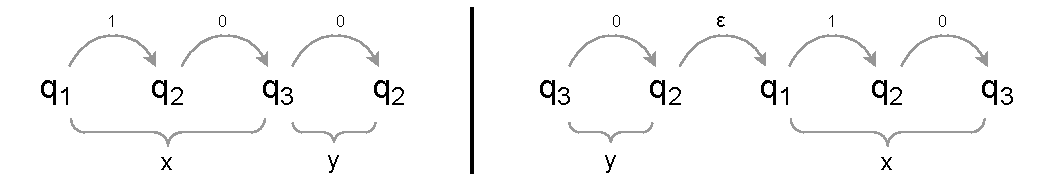
\includegraphics[scale=0.8]{Figures/Problem1.67c.pdf} \\
Comparison of state transitions between the DFA $M$ for $A$ on input string $100$ (left), \\ and how a finite automaton, say $M'$ that recognizes $RC(A)$ would compute on $010$, \\ which is a rotation of $100$ (right). \\
\end{center}

Now, let's simulate how a finite automaton $M'$ that recognizes $RC(A)$ would compute in above case:
\begin{enumerate}
\item  $M'$ starts at state $q_{3}$, and keeps on computing on the input like $M$ until an accept state is reached.
\item  When an accept state is reached, which in this case is $q_{2}$, it keeps on computing like $M$, but also takes an $\epsilon$-transition to the start state $q_{1}$.
\item After taking an $\epsilon$-transition to the start state $q_{1}$, the automaton keeps on computing as $M$, and accepts if it finishes at state  $q_{3}$.
\end{enumerate}

In general, a finite automaton $M'$ can be constructed, which recognizes $RC(A)$ by implementing above 3 points for every state in $M$.

\newpage

\begin{center}
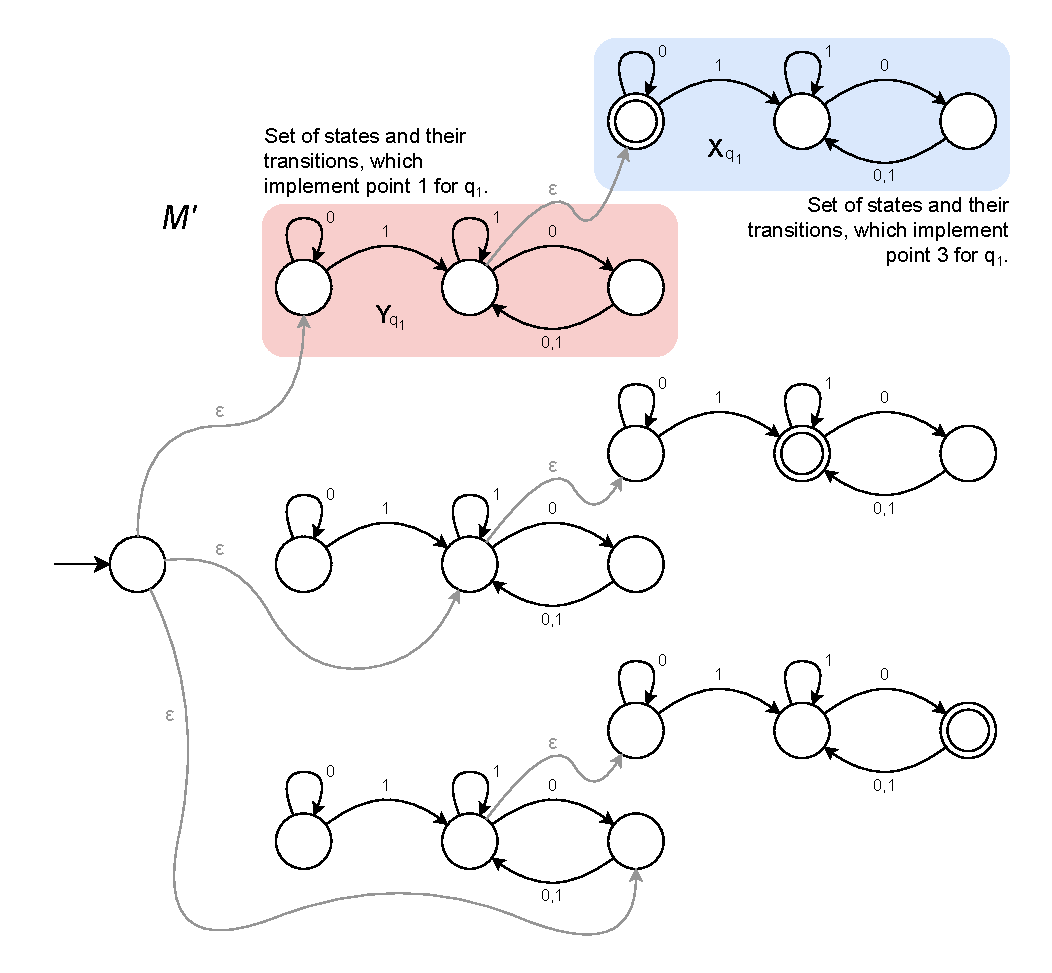
\includegraphics[scale=0.9]{Figures/Problem1.67b.pdf} \\
State diagram of DFA $M'$ that recognizes $RC(A)$. $M'$ uses two copies of $M$, which are modified to implement points 1 and 3  for each state in $M$, and the $\epsilon$-transitions implement point 2.
\end{center}
\end{idea}

\newpage

\begin{proof}
Let $M = (Q, \Sigma, \delta, q_{0}, F)$ be the DFA that recognizes $A$. Construct the NFA $M' = (Q', \Sigma, \delta', q_{0}', F')$ to recognize $RC(A)$.
\begin{enumerate}
\item $Q' = \{ q_{s} \} \cup Q_{x} \cup Q_{y}$, where
\[ 
Q_{x} = \bigcup_{i=1}^{|Q|}X_{q_{i}} \ , \ Q_{y} = \bigcup_{i=1}^{|Q|}Y_{q_{i}}
\]
For each $q_{i} \in Q$
\[ 
X_{q_{i}} = \bigcup_{j=1}^{|Q|}(q_{i}, x, q_{j}) \ , \ Y_{q_{i}} = \bigcup_{j=1}^{|Q|}(q_{i}, y, q_{j}), \ and \ each \ q_{i}, q_{j} \in Q
\]
The set $X_{q_{i}}$ is the set of states that implement point 1 for state $q_{i} \in Q$, and $Y_{q_{i}}$ is the set of states that implement point 3 for state $q_{i} \in Q$. The state $q_{s}$ is the new start state.
\item $q_{0}' = q_{s}$
\item $F' = \{ (q_{1}, x, q_{1}), (q_{2}, x, q_{2}), \cdots, (q_{n}, x, q_{n})  \}$, where each $q_{i} \in Q$.
\item Define $\delta'$(q, a) so that for any $q \in Q'$ and any $a \in \Sigma_{\epsilon}$:
\begin{center}
$\displaystyle \delta '( q,\ a) \ =\begin{cases}
\{(q_{1}, y, q_{1}), (q_{2}, y, q_{2}),\cdots,(q_{n}, y, q_{n})\} & q=q_{s} \ and\ a\ =\ \epsilon \\
\{(q_{i},x,\delta(q_{j},a))\}  & q \in Q_{x} \\
\{(q_{i},y,\delta(q_{j},a))\}  & q \in Q_{y} \ and \ q_{j} \notin F \\
\{(q_{i},y,\delta(q_{j},a))\}  & q \in Q_{y}, \ q_{j} \in F \ and \ a \neq \epsilon \\
\{(q_{i},x,q_{0})\}  & q \in Q_{y}, \ q_{j} \in F \ and \ a = \epsilon
\end{cases}$
\end{center}
\end{enumerate}
\end{proof}

\end{document}